\documentclass[12pt]{IEEEtran}
\usepackage{graphicx}
\usepackage{blindtext}
\usepackage{caption}
\usepackage{float}
\usepackage[a4paper,margin=1in,footskip=0.25in]{geometry}
\usepackage{pdfpages}

% uncomment for double spacing
%\usepackage{setspace}
%\doublespace

%\usepackage[english]{babel}
%\usepackage[style=ieee,backend=biber]{biblatex}
\usepackage[autostyle]{csquotes}
%\addbibresource{policypaper.bib}
\usepackage{hyperref}
\hypersetup{
    colorlinks,
    citecolor=black,
    filecolor=black,
    linkcolor=black,
    urlcolor=black
}

\begin{document}

\title{Some Title}
\author{
Jon Bakies, Mitchell Dunn, Elias Kapetanopoulos, and Magdy Ellabidy \\
Department of Computer Science and Networking \\
Wentworth Institute of Technology \\
Boston, MA 02115, USA \\
bakiesj@wit.edu, dunnm8@wit.edu, kapetanopoulose@wit.edu, ellabidym@wit.edu
} 

\maketitle
\newpage
\clearpage

\section{Serial Over Lan}
\subsection{ser2net}
Ser2net is a daemon that opens a TCP or Telnet connection to the server's serial ports.
After connecting all of the devices' communication ports to the Raspberry Pi ser2net allows for a single telnet connection to each device.
There are some nuances that come along with this daemon.
Ser2net does not provide a service for SSH, so the communication between the user and the device will be unencrypted.
Although SSH would be preferred, a telnet connection is acceptable because in order to access the Serial over LAN (SoL) a user has to VPN into the network.
The only way to access the network is physically or via a secure connection.
Another nuance is the configuration.
The way ser2net opens a connection to the serial ports is by the device in the /dev directory.
The devices in the /dev directory are named by the order in which they are plugged in, meaning the needs to be an order in which they are plugged in.
\subsubsection{Configuration}
The default ser2net config file is located at /etc/ser2net.conf.
The configuration file defines all of the connections ser2net provides.
An example of connection for this SoL project is \textit{192.168.1.12,5560:telnet:0:/dev/ttyUSB1:9600 8DATABITS NONE P5R3 remctl}.
It is broken into parts \textit{\textless network port\textgreater :\textless state\textgreater :\textless timeout \textgreater :\textless device\textgreater :\textless options \textgreater}.
The network port defines the end point a user will use to connect to the serial port.
The state option is used to determine the protocol used to communicate with the serial port.
The third option is the timeout in seconds.
The will be disconnected if there are this many seconds of no activity.  
This option is used to prevent inactive users from blocking others from using the device.
After timeout is the device, which as previously discussed is located in the /dev directory.
The final part is designated for options, separated by space.
Options for this project are specifically for a Cisco console device.
The P5R3 option is the name of a banner created earlier in the file that lets the user know which device they're connected to. 

\subsubsection{Installation}
ser2net is available on the apt package manger, so install is simple.

\textit{apt install ser2net}
\subsection{USB hub}
The USB hub is used to limit the wires run to the server room.
All of the devices in the pod are connected to the USB hub.
Because there are currently at most 9 devices in a pod, a 13 port hub is used.
In order to constantly have the same device number, the devices need to be plugged in a specific configuration.
Figure 1 shows a mockup of the usb hub.
Each used port is labeled with the device that is plugged into it and the phsycial port address used by the hub.
These are important to note because they are what determine ser2net's configuration.
The port number describes the physical port of the device atached, which is directly mapped to the device file.
The relationship between device and port is very important and should be standardized.

\subsection{USB-RJ45 Converter}
The USB hub is plugged into a USB to RJ45 converted to extend the connection into the server room.
The reason this is needed is because a USB cable is rated for only 5 meters in length without a repeater.
RJ45 on the other hand has a much longer rating of 100 meters, which is more than sufficient for the lab set up.
After the RJ45 line is run into the server room, it will be converted back into USB and plugged into a port on the Raspberry Pi.

\subsection{Naming Scheme}
The device names are determined by pod number, device type, and device number.
Pods are numbered 1 through 5.
For perspective, we are standing at the front of the room looking at the server room.
Pod 1 will be the left most pod that is closest to the front of the room.
The pod number will continue to increment in a left-to-right, front-to-back fashion.
Once the pod number is designated, the devices are named in a similar way.
Starting at the top most device in the front facing door (away from the server room) of the pod, devices names are incremented going to the bottom device and wrapping to the top of the back side.
The devices are designated with an S if it is a switch, and an R if it is a router.
The final device name should look like like P1S1.


\begin{figure*}[t]
	\centering
	\makebox[\textwidth]{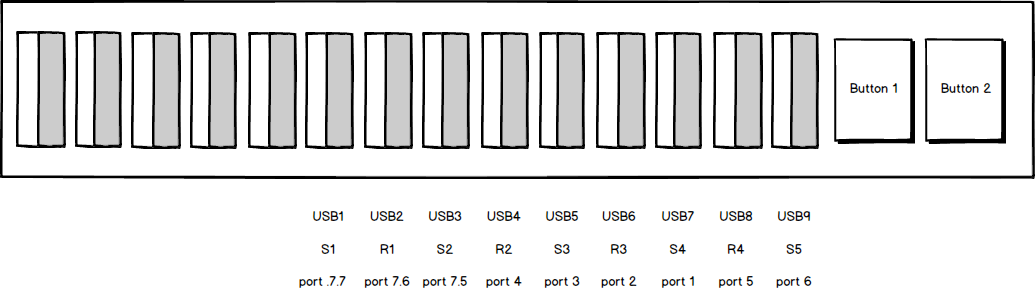
\includegraphics[width=\textwidth]{usbports.png}}
	\caption{USB hub mockup}

\end{figure*}

%\tableofcontents
%\newpage

%\newpage \section{References} \printbibliography[heading=none]
\end{document}
